\documentclass[12pt]{iopart}
\pdfoutput=1
\usepackage{iopams}
\usepackage{amssymb, epsfig}
%\usepackage{amsmath, amssymb,epsfig}
\usepackage{latexsym}

%\usepackage[hypertex,hyperindex]{hyperref}
%\usepackage{showkeys}
\usepackage{graphicx}
\usepackage{color}

\newcommand{\pf}{\mbox{pf}}
\newcommand{\vep}{\varepsilon}

\begin{document}

\bibliographystyle{plain}
\def\debproof{\noindent {\bf Proof.} }
\def\finproof{\hfill {\small $\Box$} \\}
%\renewcommand{\theequation}{\arabic{section}.\arabic{equation}}
%\tableofcontents
\makeatletter % `@' now normal "letter"
\@addtoreset{equation}{section}
\makeatother  % `@' is restored as "non-letter"
\renewcommand\theequation{{\thesection}.{\arabic{equation}}}

\title[]{Different Imaging Functions and their Numerical Tests}
\author{ }
\address{}



\maketitle

\newcommand{\eps}{\varepsilon}
\newcommand{\RR}{\mathcal{R}}
\newtheorem{lem}{Lemma}[section]
\newtheorem{prop}{Proposition}[section]
\newtheorem{cor}{Corollary}[section]
\newtheorem{thm}{Theorem}[section]
\newtheorem{rem}{Remark}[section]
\newtheorem{alg}{Algorithm}[section]
\newtheorem{assum}{Assumption}[section]
\newtheorem{definition}{Definition}[section]


\newcounter{RomanNumber}
\newcommand{\MyRoman}[1]{\rm\setcounter{RomanNumber}{#1}\Roman{RomanNumber}}

\newcommand{\bL}{\mathbf{L}}
\newcommand{\bH}{\mathbf{H}}
\newcommand{\bW}{\mathbf{W}}
\newcommand{\bP}{\mathbf{P}}
\newcommand{\bQ}{\mathbf{Q}}
\newcommand{\bp}{\mathbf{p}}
\newcommand{\bq}{\mathbf{q}}
\newcommand{\uL}{u_{_{\rm L}}}
\newcommand{\vL}{v_{_{\rm L}}}
\newcommand{\tuL}{\tilde u_{_{\rm L}}}
\newcommand{\tvL}{\tilde v_{_{\rm L}}}
\newcommand{\fL}{f_{_{\rm L}}}
\newcommand{\gL}{g_{_{\rm L}}}
\newcommand{\bpL}{\bp_{_{\rm L}}}
\newcommand{\bqL}{\bq_{_{\rm L}}}
\newcommand{\tbpL}{\tilde{\bp}_{_{\rm L}}}
\newcommand{\tbqL}{\tilde{\bq}_{_{\rm L}}}
\newcommand{\tbpLf}{\tilde{\bp}_{_{\rm L,1}}}
\newcommand{\tbpLs}{\tilde{\bp}_{_{\rm L,2}}}
\newcommand{\tbqLf}{\tilde{\bq}_{_{\rm L,1}}}
\newcommand{\tbqLs}{\tilde{\bq}_{_{\rm L,2}}}
\newcommand{\bn}{\nu}
\newcommand{\bv}{\mathbf{v}}
\newcommand{\om}{\omega}
\newcommand{\pa}{\partial}
\newcommand{\la}{\langle}
\newcommand{\ra}{\rangle}
\newcommand{\lla}{\la{\hskip -2pt}\la}
\newcommand{\rra}{\ra{\hskip -2pt}\ra}
\newcommand{\jj}{\|{\hskip -0.8pt} |}
\newcommand{\al}{\alpha}
\newcommand{\ze}{\zeta}
\newcommand{\si}{\sigma}
\newcommand{\ep}{\varepsilon}
\newcommand{\na}{\nabla}
\newcommand{\vp}{\varphi}
\newcommand{\ga}{\gamma}
\newcommand{\Ga}{\Gamma}
\newcommand{\Om}{\Omega}
\newcommand{\de}{\delta}
\newcommand{\Th}{\Theta}
\newcommand{\De}{\Delta}
\newcommand{\Lam}{\Lambda}
\newcommand{\lam}{\lambda}
\newcommand{\tri}{\triangle}
\newcommand{\lj}{[{\hskip -2pt} [}
\newcommand{\rj}{]{\hskip -2pt} ]}
\newcommand{\bks}{\backslash}
%\newcommand{\diag}{\mathrm{diag}}
\newcommand{\diam}{\mathrm{diam}}
\newcommand{\osc}{\mathrm{osc}}
\newcommand{\meas}{\mathrm{meas}}
\newcommand{\dist}{\mathrm{dist}}

\newcommand{\mL}{\mathscr{L}}
\newcommand{\cT}{{\cal T}}
\newcommand{\cM}{{\cal M}}
\newcommand{\cE}{{\cal E}}
\newcommand{\cL}{{\cal L}}
\newcommand{\cF}{{\cal F}}
\newcommand{\cB}{{\cal B}}
\newcommand{\PML}{{\rm PML}}
\newcommand{\FEM}{{\rm FEM}}
\newcommand{\rd}{\,\mathrm{d}}

\renewcommand{\i}{\mathbf{i}}
\renewcommand{\v}{\mathbf{v}}
\renewcommand{\u}{\mathbf{u}}
\renewcommand{\r}{\mathbf{r}}
\newcommand{\gR}{{\mathbb{R}}}
\newcommand{\Z}{{\mathbb{Z}}}
\newcommand{\C}{{\mathbb{C}}}
\newcommand{\I}{{\mathbb{I}}}
\renewcommand{\Re}{\mathrm{Re}\,}
\renewcommand{\Im}{\mathrm{Im}\,}
\renewcommand{\div}{\mathrm{div}}
\newcommand{\curl}{\mathrm{curl}}
\newcommand{\Curl}{\mathbf{curl}}
\newcommand{\pv}{\mathrm{p.v.}}

\newcommand{\Np}{\mathbb{N}_p}
\newcommand{\Ns}{\mathbb{N}_s}
\newcommand{\Tp}{\mathbb{T}_p}
\newcommand{\Ts}{\mathbb{T}_s}
\newcommand{\Na}{\mathbb{N}_\alpha}
\newcommand{\Nb}{\mathbb{N}_\beta}
\newcommand{\Ta}{\mathbb{T}_\alpha}
\newcommand{\Tb}{\mathbb{T}_\beta}
\newcommand{\GG}{\mathcal{G}}

\newcommand{\N}{\mathbb{N}}
\newcommand{\D}{\mathbb{D}}
\newcommand{\T}{\mathbb{T}}
\newcommand{\A}{\mathbb{A}}
\newcommand{\B}{\mathbb{B}}
\newcommand{\G}{\mathbb{G}}
\newcommand{\F}{\mathbb{F}}
\newcommand{\R}{\mathbb{R}}
\newcommand{\W}{\mathbb{W}}
\newcommand{\V}{\mathbb{V}}
\newcommand{\U}{\mathbb{U}}
\newcommand{\J}{\mathbb{J}}
\newcommand{\Zg}{\mathbb{Z}}
\newcommand{\Gtheta}{\mathbb{\Theta}}
\newcommand{\Gphi}{\mathbb{\Phi}}

%%%%%%%%%%%%%%%%%%%%%%%%%%%%%%%%%%%%%%%%%%%%%%%%%%%%%%%%%%%%%%%%%%%%
\newcommand{\be}{\begin{eqnarray}}
\newcommand{\ee}{\end{eqnarray}}
\newcommand{\ben}{\begin{eqnarray*}}
	\newcommand{\een}{\end{eqnarray*}}
\newcommand{\nn}{\nonumber}



\ben
\hskip-1cm I_1(z)=\Im\sum_{q=e_1,e_2}\int_{\Gamma_0^d}\int_{\Gamma_0^d}\,
[\T_D(x_s,z)^Tq]\cdot[\T_D(x_r,z)^T\overline{u^s_q(x_r,x_s)}]\,ds(x_r)ds(x_s).
\een
\begin{figure}[!h]
	\centering
	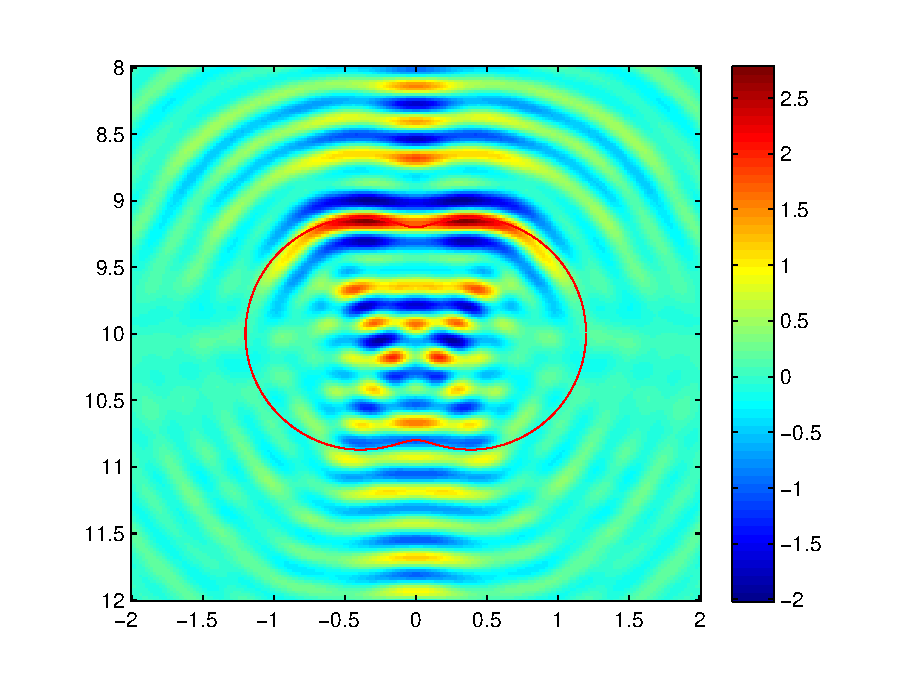
\includegraphics[width=0.67\textwidth]{./figures/fullwave}
	\caption{$I_1$}\label{I1}
\end{figure}
\ben
\hskip-1cm I_2(z)=\Im\int_{\Gamma_0^d}\int_{\Gamma_0^d}\,
\i[\frac{\pa \Phi^s(x_s,z)}{\pa x_2(x_s)}]\nabla_z\times[\T_D(x_r,z)^T\overline{u^s_{e_2}(x_r,x_s)}]\,ds(x_r)ds(x_s).
\een
\begin{figure}[!h]
	\centering
	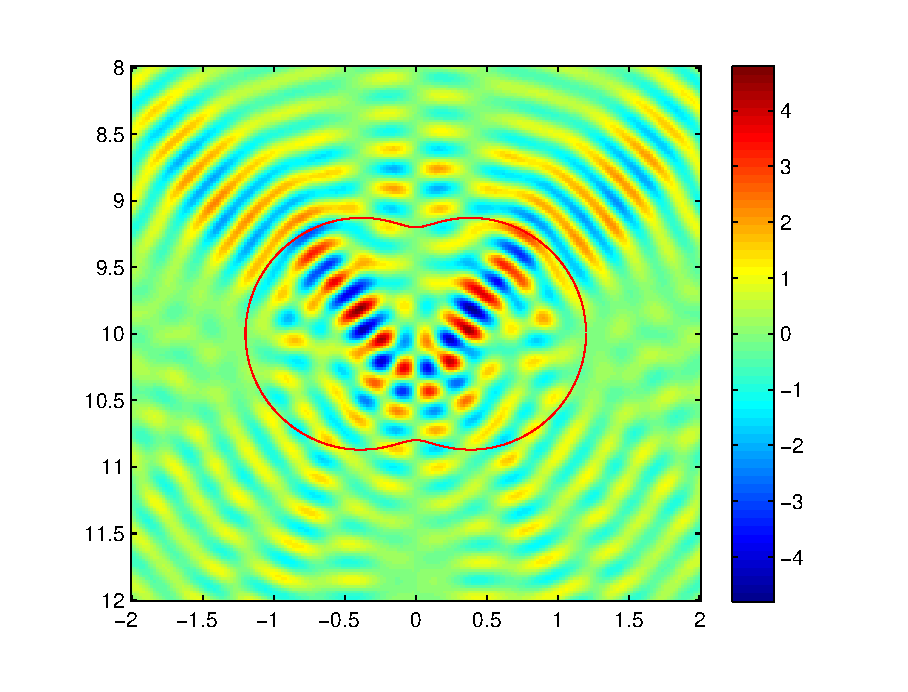
\includegraphics[width=0.67\textwidth]{./figures/ks_Spotential_e2}
	\caption{$I_2$}\label{I2}
\end{figure}
\ben
\hskip-1cm I_3(z)=\Im\int_{\Gamma_0^d}\int_{\Gamma_0^d}\,
\i[\frac{\pa \Phi^p(x_s,z)}{\pa x_2(x_s)}]\nabla_z\times[\T_D(x_r,z)^T\overline{u^s_{e_2}(x_r,x_s)}]\,ds(x_r)ds(x_s).
\een
\begin{figure}[!h]
	\centering
	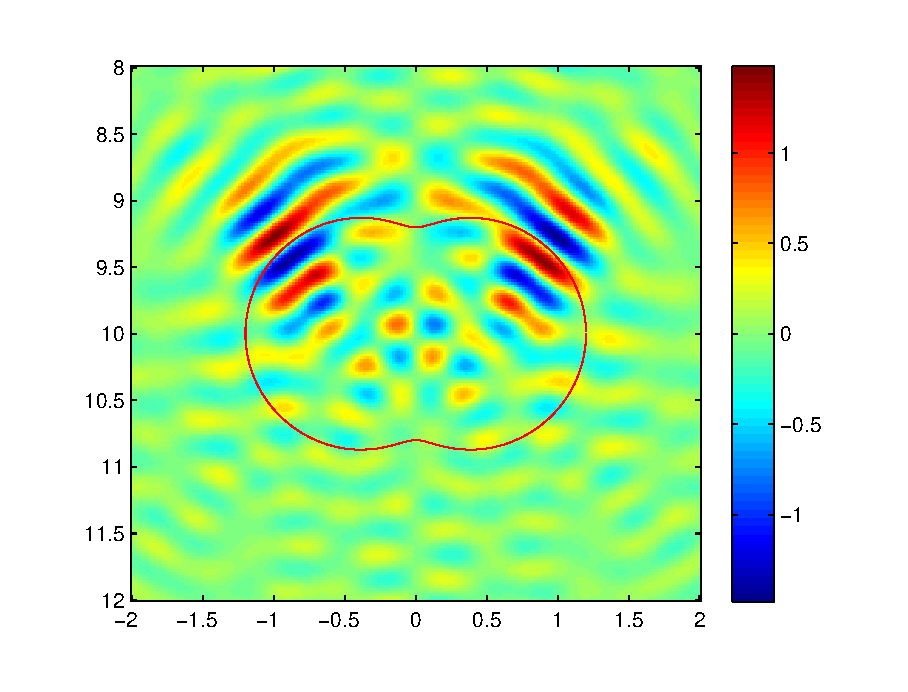
\includegraphics[width=0.7\textwidth]{./figures/kp_Spotential_e2}
	\caption{$I_3$}\label{I3}
\end{figure}
\ben
\hskip-1cm I_4(z)=\Im\int_{\Gamma_0^d}\int_{\Gamma_0^d}\,
\i[\frac{\pa \Phi^s(x_s,z)}{\pa x_2(x_s)}]\nabla_z\cdot[\T_D(x_r,z)^T\overline{u^s_{e_2}(x_r,x_s)}]\,ds(x_r)ds(x_s).
\een
\begin{figure}[!h]
	\centering
	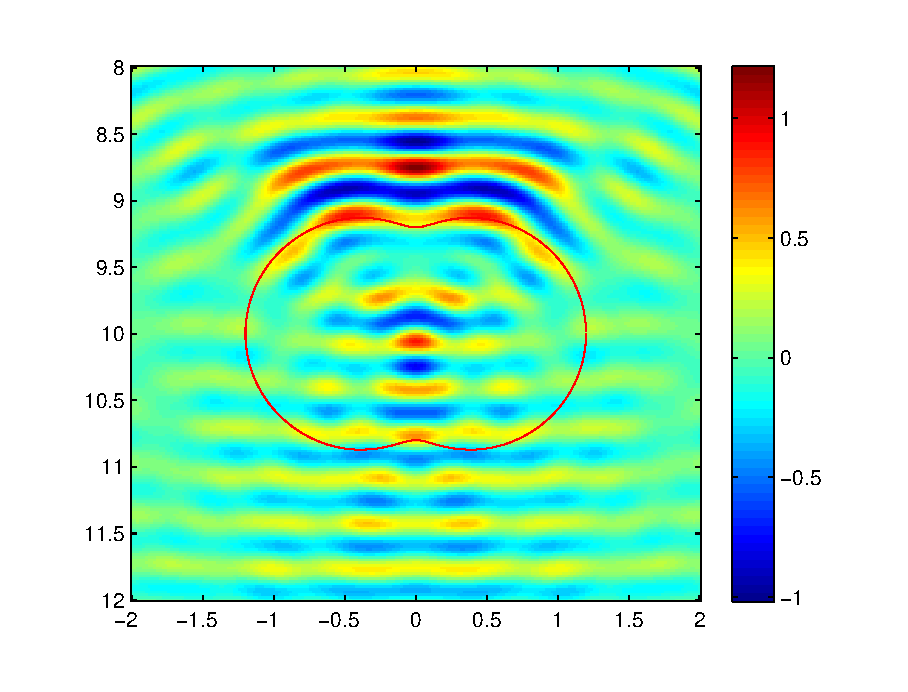
\includegraphics[width=0.7\textwidth]{./figures/ks_Ppotential_e2}
	\caption{$I_4$}\label{I4}
\end{figure}
\ben
\hskip-1cm I_5(z)=\Im\int_{\Gamma_0^d}\int_{\Gamma_0^d}\,
\i[\frac{\pa \Phi^p(x_s,z)}{\pa x_2(x_s)}]\nabla_z\cdot[\T_D(x_r,z)^T\overline{u^s_{e_2}(x_r,x_s)}]\,ds(x_r)ds(x_s).
\een
\begin{figure}[!h]
	\centering
	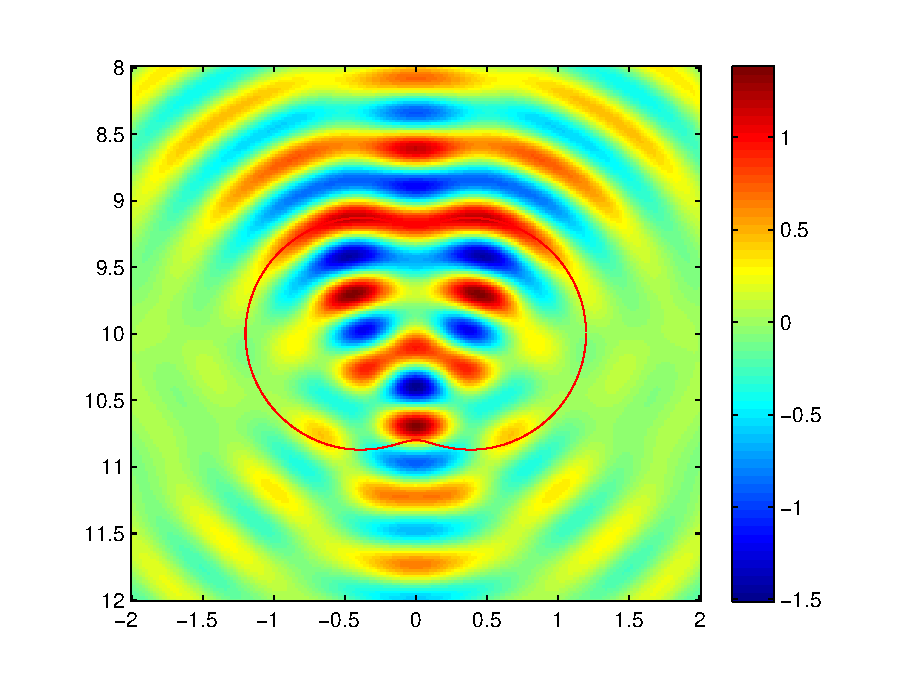
\includegraphics[width=0.7\textwidth]{./figures/kp_Ppotential_e2}
	\caption{$I_5$}\label{I5}
\end{figure}
\ben
\hskip-1cm I_6(z)=\Im\int_{\Gamma_0^d}\int_{\Gamma_0^d}\,
\i[\frac{\pa \Phi^s(x_s,z)}{\pa x_2(x_s)}]\nabla_z\times[\T_D(x_r,z)^T\overline{u^s_{e_1}(x_r,x_s)}]\,ds(x_r)ds(x_s).
\een
\begin{figure}[!h]
	\centering
	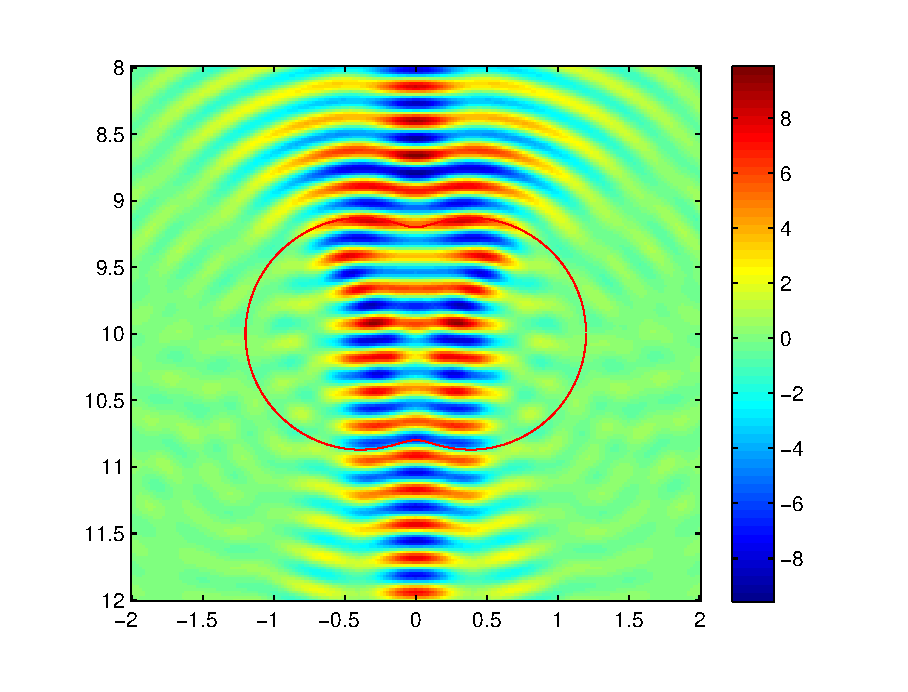
\includegraphics[width=0.7\textwidth]{./figures/ks_Spotential_e1}
	\caption{$I_6$}\label{I6}
\end{figure}
\ben
\hskip-1cm I_7(z)=\Im\int_{\Gamma_0^d}\int_{\Gamma_0^d}\,
\i[\frac{\pa \Phi^s(x_s,z)}{\pa x_2(x_s)}]\nabla_z\times[\T_D(x_r,z)^T\overline{u^s_{e_1}(x_r,x_s)}]\,ds(x_r)ds(x_s).
\een
\begin{figure}[!h]
	\centering
	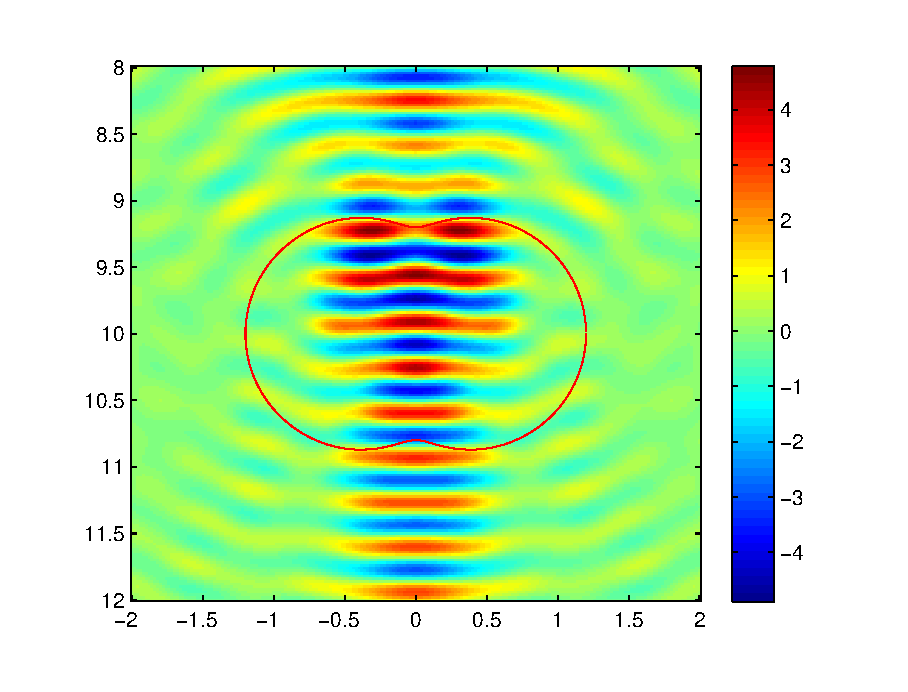
\includegraphics[width=0.7\textwidth]{./figures/kp_Spotential_e1}
	\caption{$I_7$}\label{I7}
\end{figure}
\ben
\hskip-1cm I_8(z)=\Im\int_{\Gamma_0^d}\int_{\Gamma_0^d}\,
\i[\frac{\pa \Phi^s(x_s,z)}{\pa x_2(x_s)}+\frac{\pa \Phi^p(x_s,z)}{\pa x_2(x_s)}]\nabla_z\cdot[\T_D(x_r,z)^T\overline{u^s_{e_2}(x_r,x_s)}]\,ds(x_r)ds(x_s).
\een
\begin{figure}[!h]
	\centering
	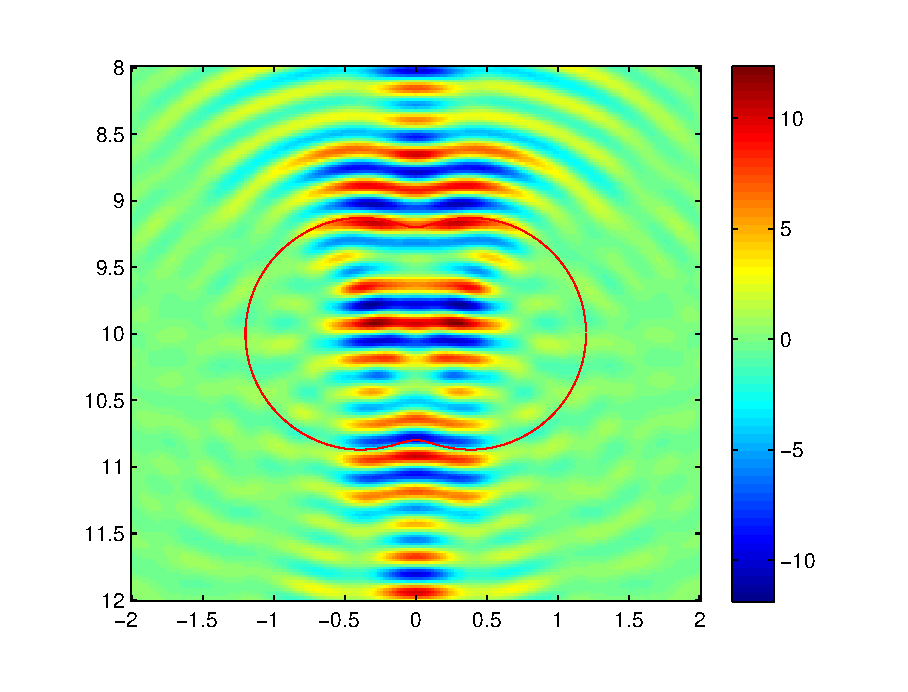
\includegraphics[width=0.7\textwidth]{./figures/ks_add_kp_Spotential_e1}
	\caption{$I_8$}\label{I8}
\end{figure}
\ben
\hskip-1cm I_9(z)=\Im\int_{\Gamma_0^d}\int_{\Gamma_0^d}\,
\i[\frac{\pa \Phi^s(x_s,z)}{\pa x_2(x_s)}+\frac{\pa \Phi^p(x_s,z)}{\pa x_2(x_s)}]\nabla_z\times[\T_D(x_r,z)^T\overline{u^s_{e_1}(x_r,x_s)}]\,ds(x_r)ds(x_s).
\een
\begin{figure}[!h]
	\centering
	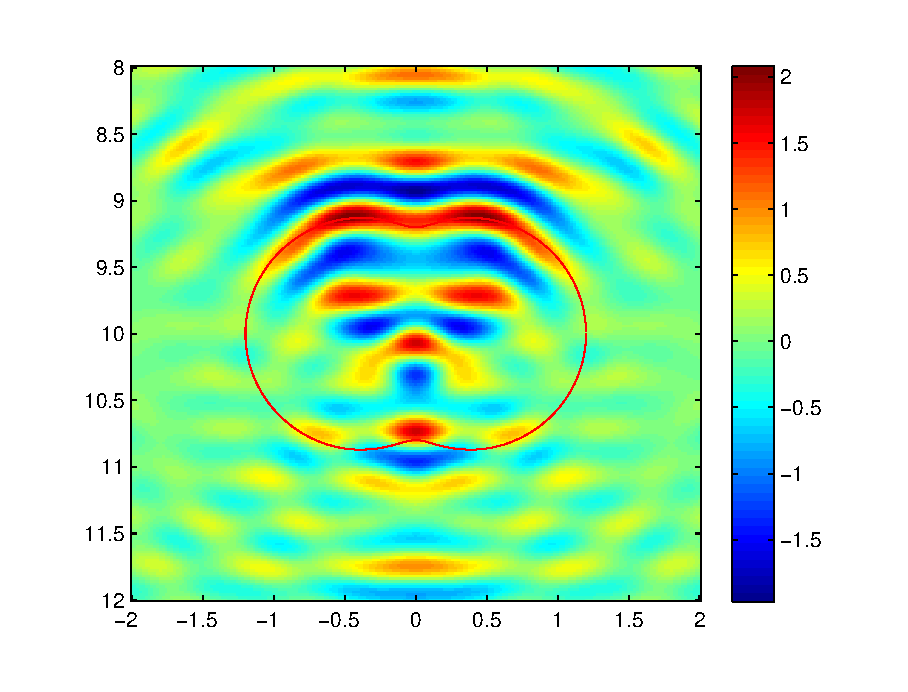
\includegraphics[width=0.7\textwidth]{./figures/ks_add_kp_Ppotential_e2}
	\caption{$I_9$}\label{I9}
\end{figure}
\ben
\hskip-1cm
I_{10}(z)=\frac{c_s}{k_s}I_8(z)+\frac{c_p}{k_p}I_9(z)
\een
\begin{figure}[!h]
	\centering
	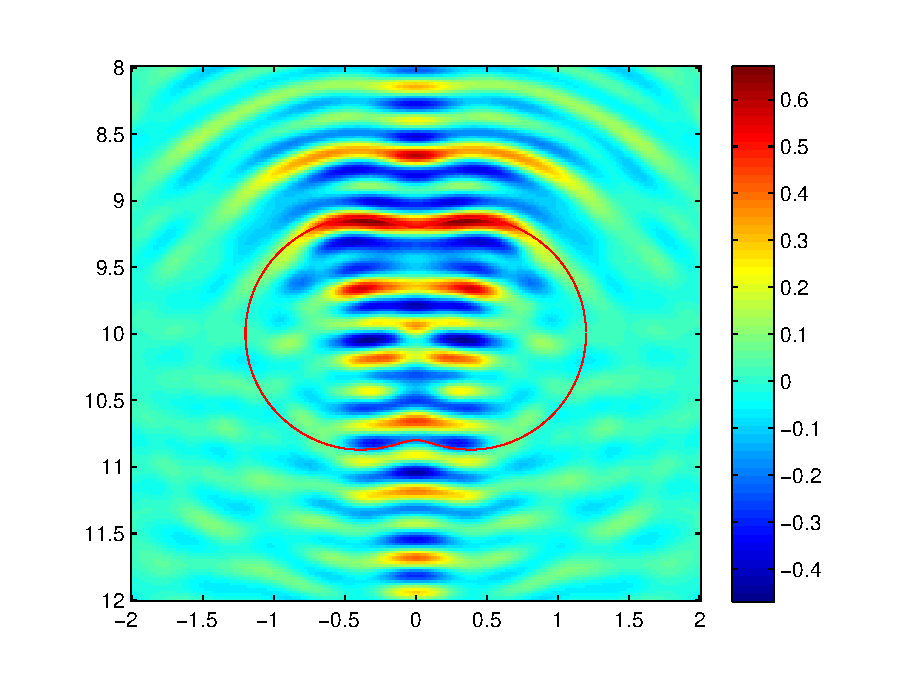
\includegraphics[width=0.72\textwidth]{./figures/ks_add_kp_Spotential_e1_add_Ppotential_e2}
	\caption{$I_{10}$}\label{I10}
\end{figure}
\ben
\hskip-1cm I_{11}(z)=\Im\int_{\Gamma_0^d}\int_{\Gamma_0^d}\,
\frac{\pa \Phi^p(x_s,z)}{\pa x_2(x_s)}\frac{\pa \Phi^p(x_r,z)}{\pa x_2(x_r)}[\overline{u^s_{e_2}(x_r,x_s)}\cdot e_2]\,ds(x_r)ds(x_s).
\een
\begin{figure}[!h]
	\centering
	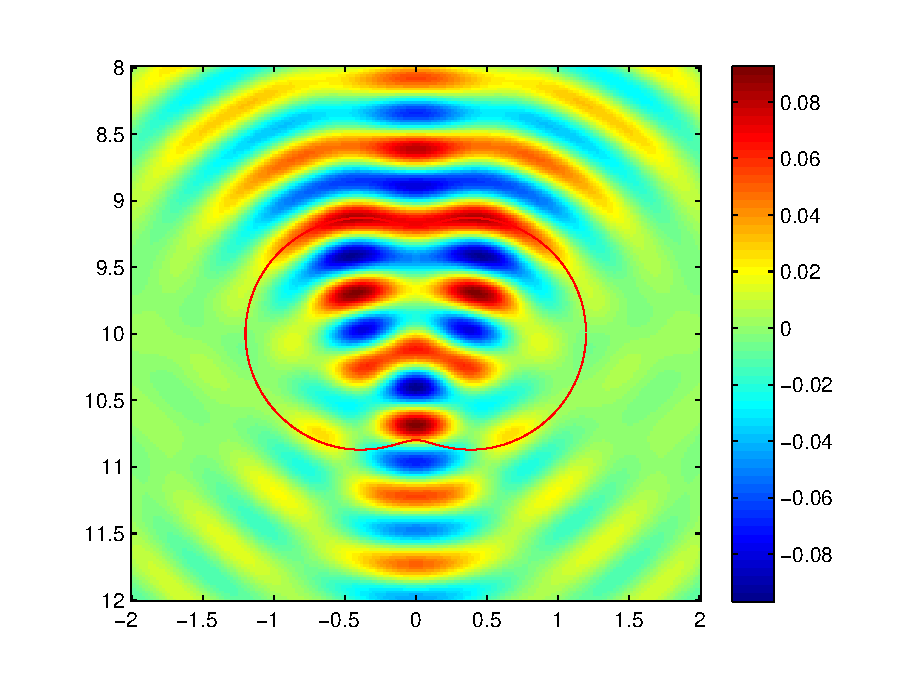
\includegraphics[width=0.7\textwidth]{./figures/kp_scalar_e2_e2}
	\caption{$I_{11}$}\label{I11}
\end{figure}
\ben
\hskip-1cm I_{12}(z)=\Im\int_{\Gamma_0^d}\int_{\Gamma_0^d}\,
\frac{\pa \Phi^s(x_s,z)}{\pa x_2(x_s)}\frac{\pa \Phi^s(x_r,z)}{\pa x_2(x_r)}[\overline{u^s_{e_1}(x_r,x_s)}\cdot e_1]\,ds(x_r)ds(x_s).
\een
\begin{figure}[!h]
	\centering
	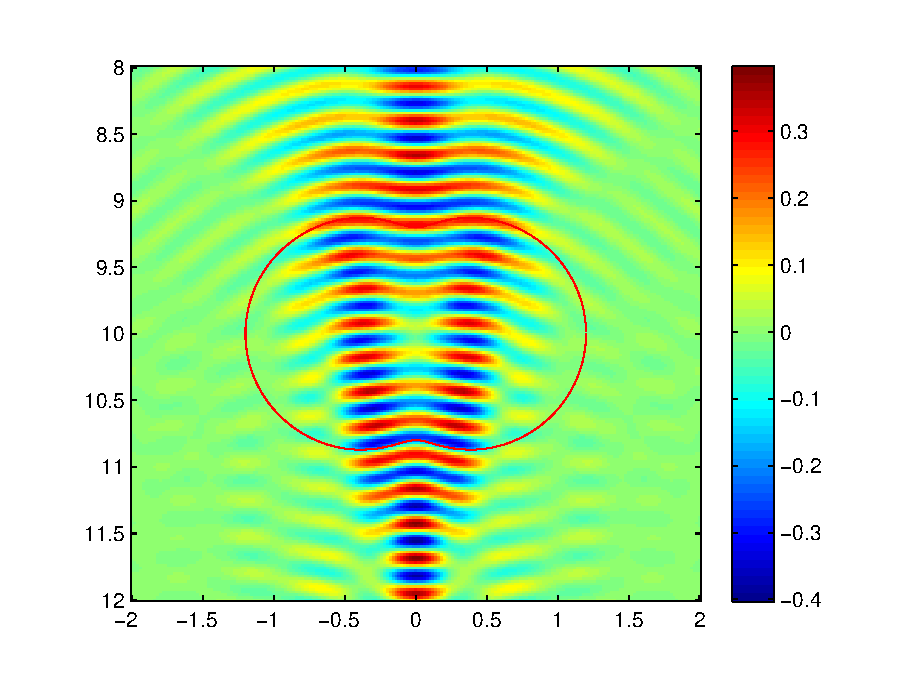
\includegraphics[width=0.7\textwidth]{./figures/ks_scalar_e1_e1}
	\caption{$I_{12}$}\label{I12}
\end{figure}
\ben
\hskip -2cm
 I_{13}(z)=\Im\int_{\Gamma_0^d}\int_{\Gamma_0^d}\,
[\frac{\pa \Phi^p(x_s,z)}{\pa x_2(x_s)}+\frac{\pa \Phi^s(x_s,z)}{\pa x_2(x_s)}][\frac{\pa \Phi^p(x_r,z)}{\pa x_2(x_r)}+\frac{\pa \Phi^s(x_r,z)}{\pa x_2(x_r)}][\overline{u^s_{e_2}(x_r,x_s)}\cdot e_2]\,ds(x_r)ds(x_s).
\een
\begin{figure}[!h]
	\centering
	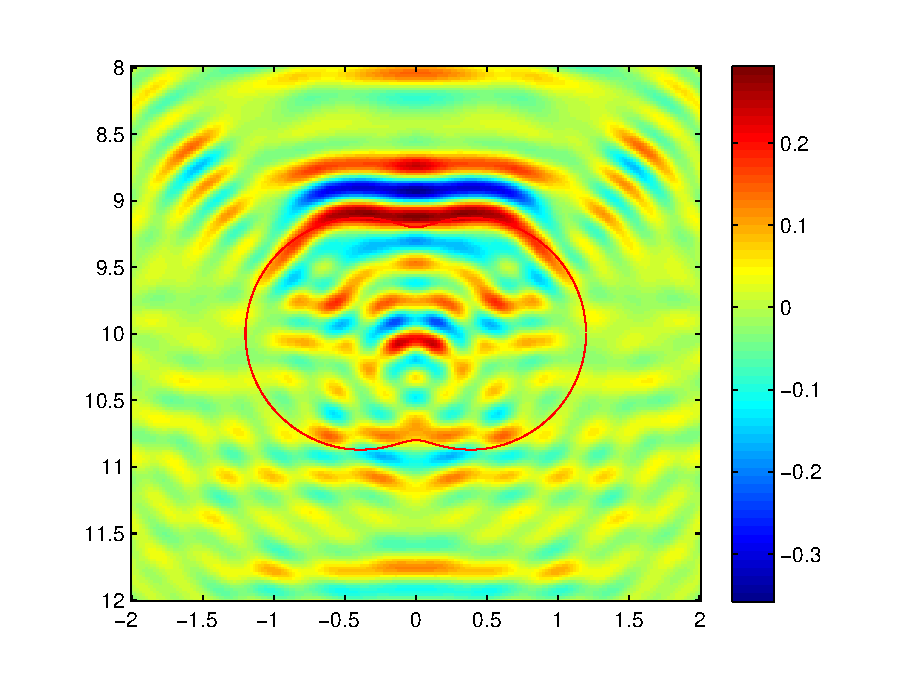
\includegraphics[width=0.72\textwidth]{./figures/ks_add_kp_scalar_e2_e2}
	\caption{$I_{13}$}\label{I13}
\end{figure}
\ben
\hskip -2cm
I_{14}(z)=\Im\int_{\Gamma_0^d}\int_{\Gamma_0^d}\,
[\frac{\pa \Phi^p(x_s,z)}{\pa x_2(x_s)}+\frac{\pa \Phi^s(x_s,z)}{\pa x_2(x_s)}][\frac{\pa \Phi^p(x_r,z)}{\pa x_2(x_r)}+\frac{\pa \Phi^s(x_r,z)}{\pa x_2(x_r)}][\overline{u^s_{e_1}(x_r,x_s)}\cdot e_1]\,ds(x_r)ds(x_s).
\een
\begin{figure}[!h]
	\centering
	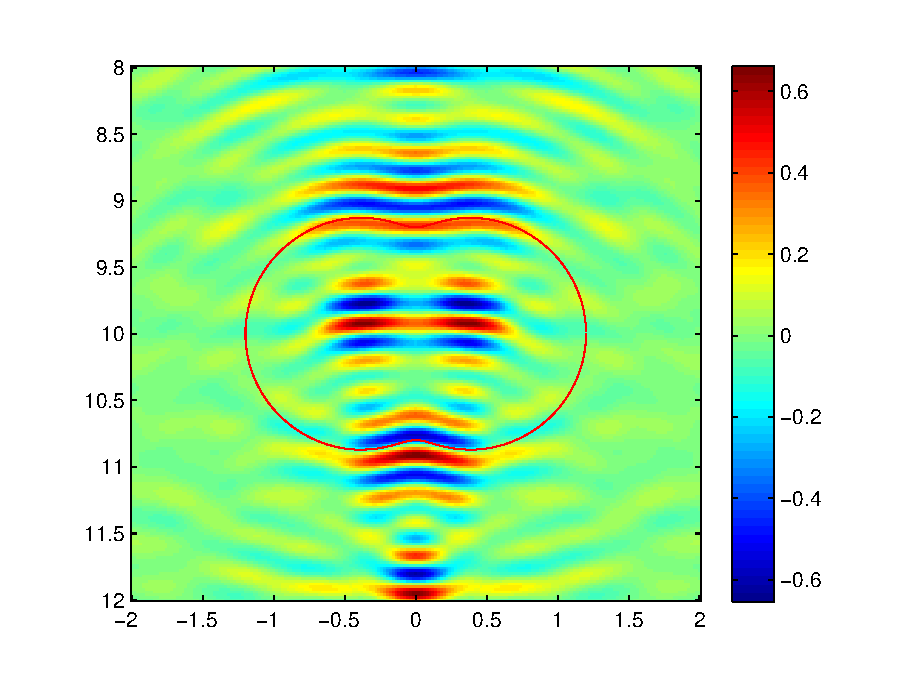
\includegraphics[width=0.72\textwidth]{./figures/ks_add_kp_scalar_e1_e1}
	\caption{$I_{14}$}\label{I14}
\end{figure}
\ben
\hskip -2cm
I_{15}(z)=c_p^2 I_{13}(z)+c_s^2I_{14}.
\een
\end{document}
